\section{Related work}

Photo retouching has been explored in image processing and computer vision communities across different domains, such as photo enhancement and image-to-image translation. Below, we first discuss recent methods on photo enhancement and then image-to-image map definitions with a main focus on learning-based methods.

\subsection{Digital photo enhancement}
% \myworries{Check Rafals' paper -- is it global tone mapping, where to put it in the related work}
\paragraph{Global image enhancement.} Colour and tone transfer is considered as a very effective technique to improve the perceptual quality of photos with pre-defined rules or examples \cite{Faridul14ASurvey, mustafa2022distilling}.

Earlier methods typically apply global changes and adjust image statistics \cite{Bychkovsky11Learning, Bae06Two, Pitie05NDimensional, Pitie07Automated, Reinhard01Color, Sunkavalli10Multi, he2020conditional, park2018distort}, e.g., mean and standard deviation, without considering image content and local variations \cite{CohenOr06Color}. These methods, in general, transfer colour changes, ignoring edits in fine details. On the other hand, our method learns a mapping per frequency band, capturing transfers even in high frequencies. \citeauthor{Bychkovsky11Learning} \cite{Bychkovsky11Learning} collected the MIT-Adobe FiveK dataset of 5,000 photographs and their retouched versions produced by five different artists. They propose a regression model to learn artists' retouching styles from before-and-after pairs. \citeauthor{chen2017fast} \cite{chen2017fast} introduce a fully-convolutional neural network model to learn global image processing operators, such as photographic style, nonlocal dehazing, and pencil drawing. \citeauthor{Hu18Exposure} \cite{Hu18Exposure} present a photo retouching pipeline for various post-processing operations, where global adjustment curves are approximated. They propose a deep reinforcement learning approach to model users' edit preferences from a given photo collection.
 
Nevertheless, global transfers cannot capture local and regional variations in a photo \cite{CohenOr06Color}. They may introduce artifacts if the local target regions of the example and input images do not match. In this method, we adapt the mappings for each image patch separately, thus accurately capturing local edits in intricate details.

\paragraph{Local context-aware image enhancement.} 
To capture local variations, different methods have been proposed, such as learning local representative color transforms \cite{kim2021representative}, estimating an image-to-illumination mapping with a local feature extractor \cite{wang2019underexposed}, local histogram matching \cite{Shapira13Image}, segmentation \cite{Laffont14Transient,Tai07Soft}, combining and learning pre-defined filters \cite{Berthouzoz11AFramework,Chen18Deep,Huang14Parametric,Omiya18Learning,Saeedi18Multimodal} or with further user guidance \cite{An10User,Pouli11Progressive,Tai05Local}, detection or learning of image semantics and context \cite{Gharbi17Deep,Hwang12Context,Kaufman12Content,Nam17Deep,Yan14Automatic,Zhu18Automatic}, matching \cite{HaCohen11Nonrigid}, or precise alignment \cite{Kagarlitsky09Piecewise, Shih13Data}.

Furthermore, recent work has focused on learning global and local adjustments using spatially varying filters \cite{moran2020deeplpf, Gharbi17Deep, chen2018deep, shaham2021spatially, li2020lapar}. \citeauthor{chen2018deep} \cite{chen2018deep} introduce a global feature extraction layer along with per-pixel adjustments to enhance photos. Bilateral guided joint upsampling \cite{chen2016bilateral} also allows for local and global image processing with an encoder-decoder approach. HDRNet \cite{Gharbi17Deep} learns content-aware, global, and local adjustments via a two-stream convolutional architecture, which extracts local and global features separately to fit local affine transformations and encode the high-level description of images, respectively. Additionally, \citeauthor{moran2020deeplpf} \cite{moran2020deeplpf} propose to learn the parameters of three different spatially varying filters to automatically enhance photos.

Local colour and tone adjustments may still be insufficient to capture intricate details \cite{Bae06Two}. The transfer of such details typically requires a dense matching \cite{HaCohen11Nonrigid} or alignment between example and input images \cite{Shih14Style}. To achieve either dense matching or alignment, methods constrain their datasets to include very similar example and input images, for example, faces that have similar characteristics and views~\cite{Shih14Style}. On the other hand, this framework does not require dense correspondences between input and example images but still manages to transfer intricate details. It accurately represents such complex mappings with an operator summing the effects of various transformations multiplied by corresponding patch-adaptive weights, applied at multiple frequency bands.

\paragraph{Differentiable image processing pipelines.} To have more flexibility and control over the rendering process, methods based on image signal processors (\gls{ISP}s) have been proposed to enhance photos. Both \citeauthor{tseng2019hyperparameter}\cite{tseng2019hyperparameter} and \citeauthor{yu2021reconfigisp}\cite{yu2021reconfigisp}optimise the \gls{ISP} hyperparameters. Different from \citeauthor{tseng2019hyperparameter} \cite{tseng2019hyperparameter}, whose method is only applied to a fixed pipeline, \citeauthor{yu2021reconfigisp} \cite{yu2021reconfigisp} can explore different \gls{ISP} architectures. Furthermore, \citeauthor{tseng2022neural} \cite{tseng2022neural} model a commercial raw processing pipeline with a series of neural networks to render \gls{sRGB} images from raw data. As we expect example and input images to be processed RGB images instead of raw data, I refrain from comparing our method with such \gls{ISP}-based methods.

\subsection{Defining maps between images}

\paragraph{Unsupervised methods.} Some learning-based techniques only require one or more examples of retouched photos without their corresponding before examples to learn the transfer. Such unsupervised methods capture a certain style by decomposing images into a reflection map and an illumination map~\cite{ma2021retinexgan}, extracting and recomposing band representations of training images~\cite{yang2020fidelity}, regularising unpaired training using information extracted from the input~\cite{9334429}, segmenting the image into semantic regions~\cite{Liu16Makeup}, adaptive image regions~\cite{Frigo16Split}, learning semantic and global features~\cite{Chen18Deep}, progressively translating images from coarse to fine via pyramids of generative models \cite{lin2020tuigan}, or utilising artistic principles and pre-defined filters~\cite{Zhang13Style,Hu18Exposure}. These methods transfer pre-defined elements of the desired style, or global colour and tone. Defining the desired style and the content of the input image that is to remain is challenging. Hence, these methods typically assume prior knowledge of the type of desired adjustments. Even so, capturing retouching edits in detail remains out of scope, as these methods are primarily designed for domain transfer, focusing on high-level features.

% TuiGAN: compare with our work, discuss how bady they perform in details although they work as single-shot --

As a weakly supervised method, \citeauthor{visual_attribute} \cite{visual_attribute} propose a technique based on image analogy \cite{Hertzmann01Image} to transfer the visual attributes, such as colour, tone, texture, and style, across images that look very different but share similar semantic structures. Similar to this work, they also work with one example pair (A and B') to transfer the attributes. However, they instead focus on high-level features, disregarding the edits in intricate details.

\paragraph{Supervised methods.} 
For a conceivable representation, many supervised transfer methods often require a large dataset of well-aligned example image pairs whose contents are very similar \cite{kim2021representative, wang2019underexposed}. However, finding or generating such a dataset is difficult, as the content of images can change dramatically. Even with such a dataset, segmentation errors, unseen semantic regions, or the image content can still significantly affect the results \cite{10.1145/2790296}. In contrast, our framework allows users to select the example pairs from which the desired style is learned, hence sidestepping the challenging semantics problem. Similar content and structures between example and input images lead to more natural transfers.

Convolutional neural networks (\gls{CNN}s) are the de facto model for image processing using supervised learning methods. While \gls{CNN}s present state-of-the-art results in computer vision tasks, they are not strictly necessary \cite{tolstikhin2021mlp}. \gls{MLP}-based architectures have recently gained popularity in image classification and image-to-image translation. \citeauthor{cazenavette2021mixergan} \cite{cazenavette2021mixergan} propose the \gls{MLP}-Mixer architecture that only uses simple \gls{MLP} blocks to learn image classification. \citeauthor{cazenavette2021mixergan} \cite{cazenavette2021mixergan} have also recently shown an application of an \gls{MLP}-based architecture for image synthesis. They adapt the \gls{MLP}-Mixer architecture \cite{tolstikhin2021mlp} to perform unpaired image-to-image translation. The fact that \gls{MLP}-based architectures attain competitive results in challenging vision tasks motivated me to explore the use of an \gls{MLP} block as an alternative to \gls{CNN}s in the context of photo retouching.

\section{Overview and motivations}
\label{chap:motivations}

Given a pair of example images $X$ and $Y$, the aim is to learn a map $M$ such that $Y = M(X)$. The learned map can subsequently be applied to a new input image $I$ to obtain the retouched output $O = M(I)$.

The map is defined by: 1) decomposing the example images into multiple feature maps $X_l$, $Y_l$ capturing details at different scales, such as coefficients at different bands of a Laplacian pyramid; 2) learning a separate mapping $M_l$ for each $X_l$, $Y_l$ pair in the patch space as a blending of transformation matrices with neural field-based weights, all learned jointly. The overall map representation is illustrated in Figure~\ref{fig:modelT}.

For the transfer of edits, the $M_l$ are computed and applied to each patch of the decomposition $I_l$ of an input image $I$ to obtain the corresponding output patch. The patches are finally placed at their spatial locations and averaged to reconstruct each band $O_l$, which are summed to obtain the output image $O$. 
%$O_l$
The motivation behind designing such a map representation with frequency decomposition and transformation blending stems from an examination of the nature of retouching edits.

\begin{itemize}
\item First, artists often decompose images into different frequency bands to gain better control over structural and textural edits of details. For instance, they filter out the low-frequency components to enhance the details more effectively (Figure \ref{fig:PS-high-pass}).

\begin{figure}[ht]
\centering
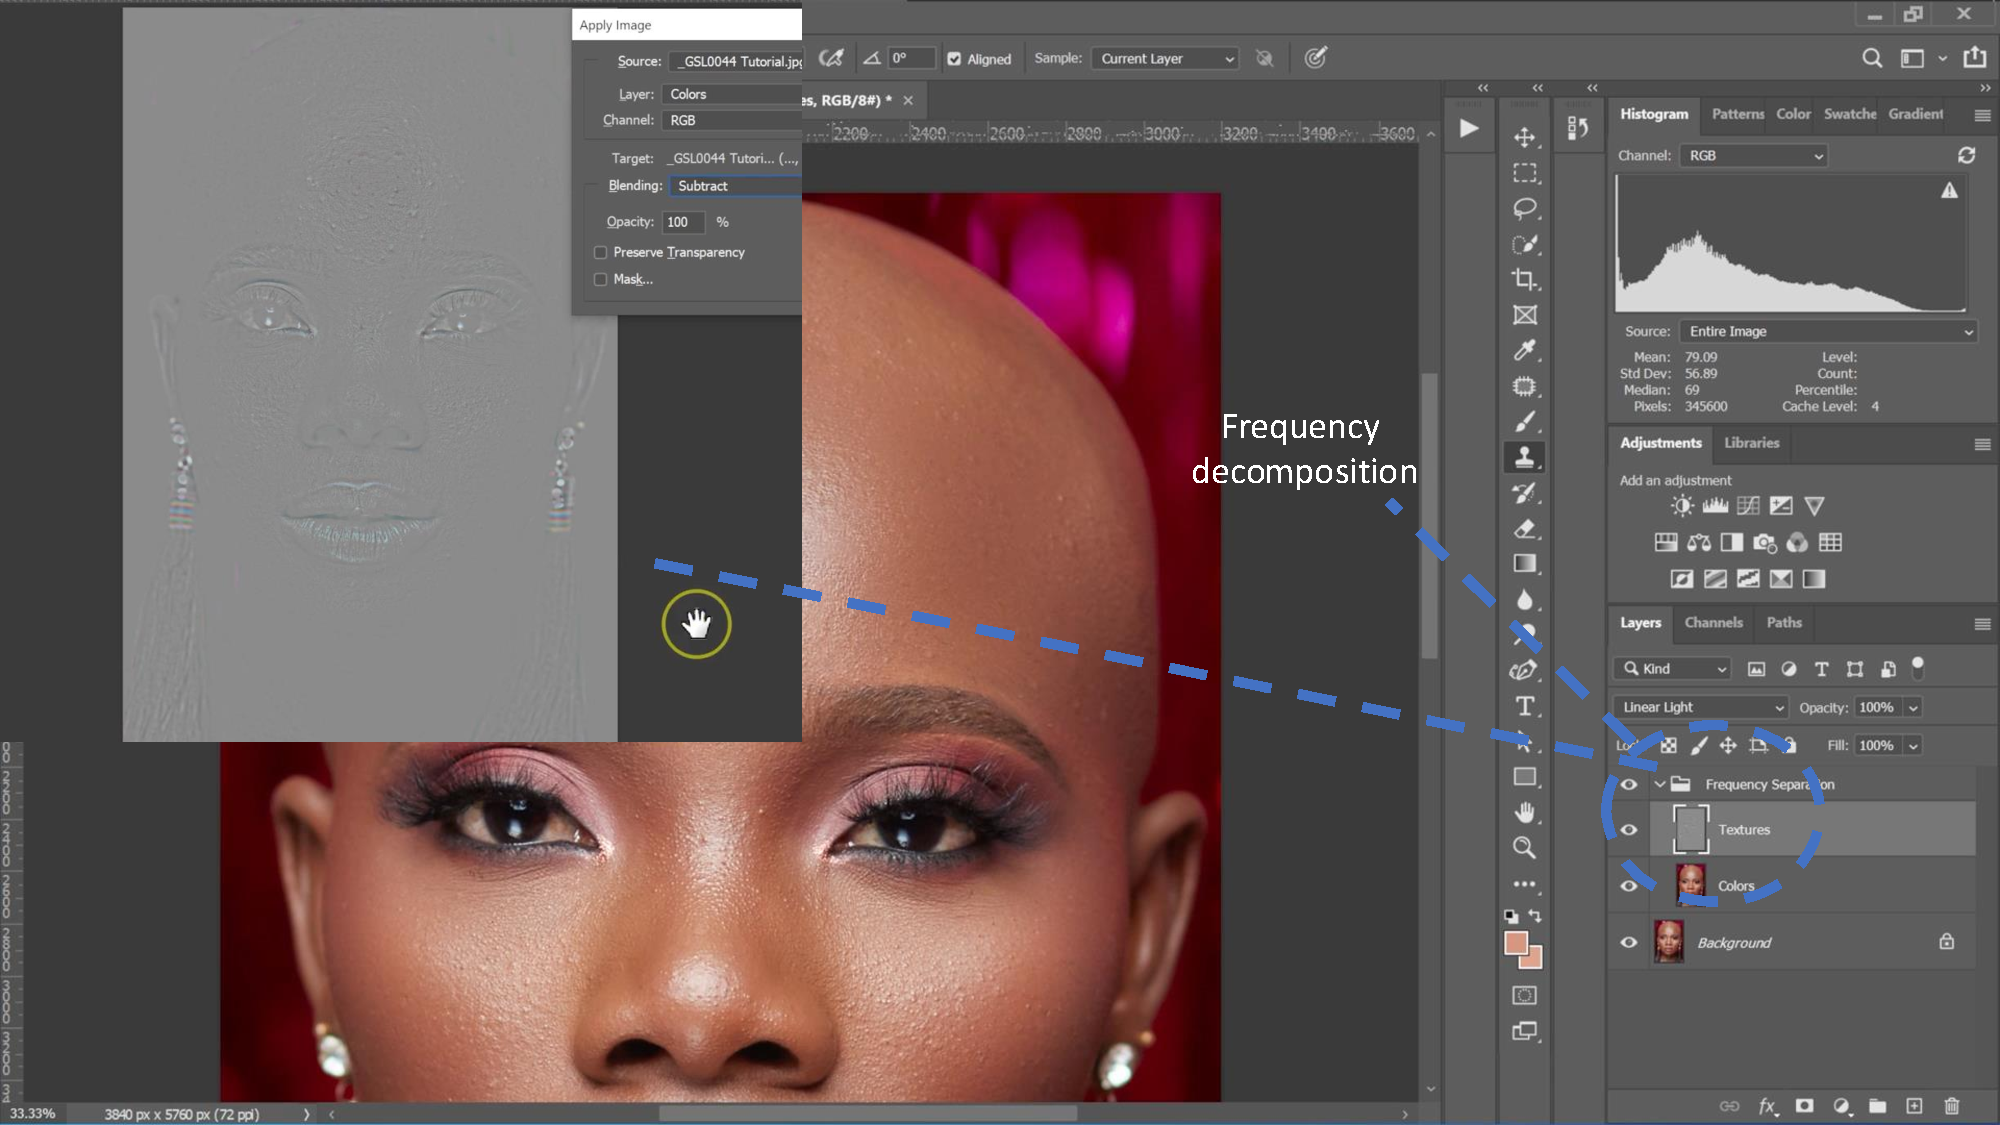
\includegraphics[width=\columnwidth]{Chapters/detail-retouching-figs/PS1.pdf}
    \caption{Frequency decomposition allows artists to have a better control over the different frequency components. Here, the layer in the top-left corner is obtained through high-pass filtering of the portrait in the background. Screenshots from [Eustace Kanyanda, 2022].}

\label{fig:PS-high-pass}
\end{figure}
\item Second, image patches of similar content, e.g. skin or hair, are retouched in a similar manner. This implies that similar patches in the patch space result in similar edits. The proposed representation leads to different transformations for patches with varying content. Local filters can offer such edits, where similar content, such as pores, transforms into another similar content, like a smooth texture (Figure \ref{fig:PS-brush}).

\begin{figure}[H]
\centering
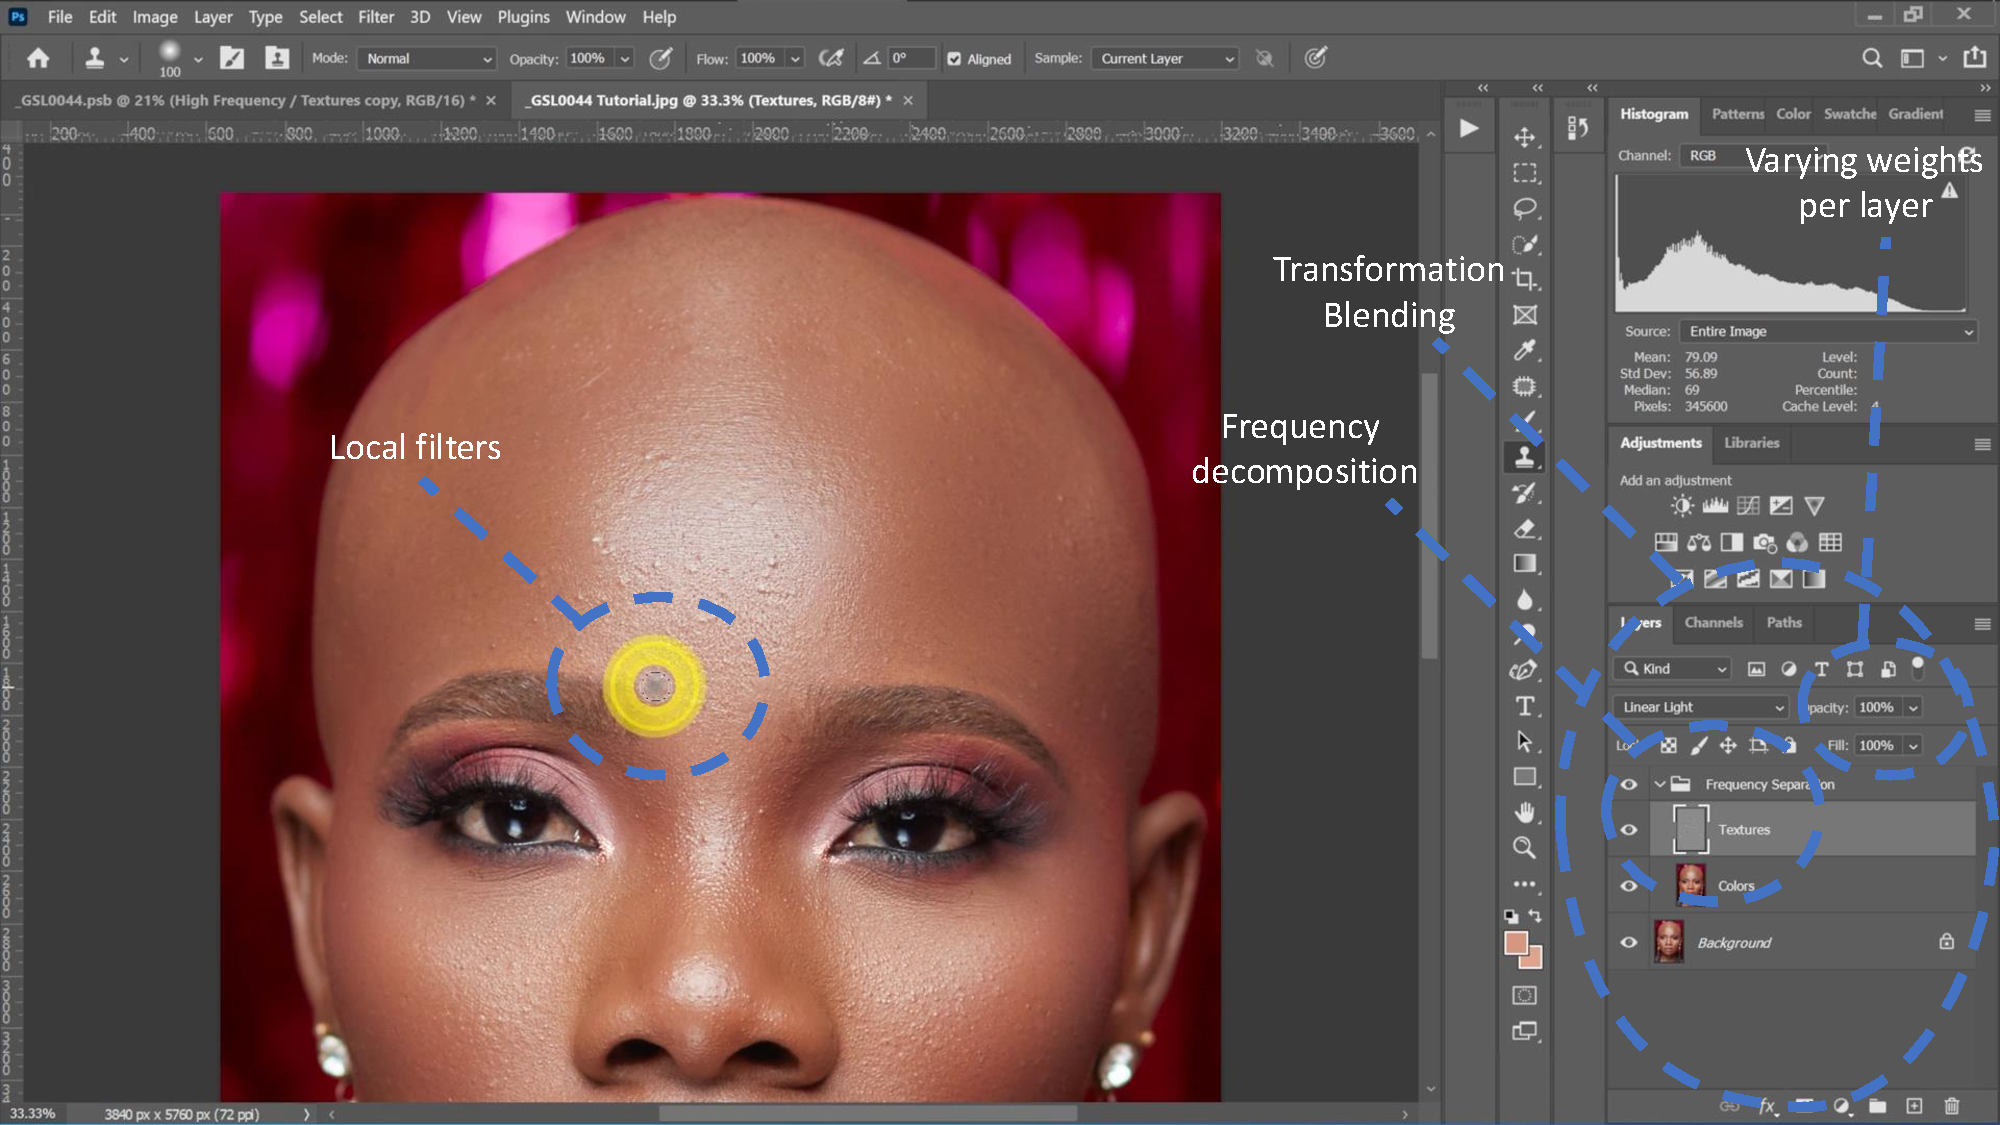
\includegraphics[width=\columnwidth]{Chapters/detail-retouching-figs/PS3.pdf}
    \caption{Local filters, such as brushes, help smooth the skin by removing undesired pores from the face. However, it is a tedious task for artists, as it requires them to address each visible pore individually.}

\label{fig:PS-brush}
\end{figure}

\begin{figure}[H]
\centering
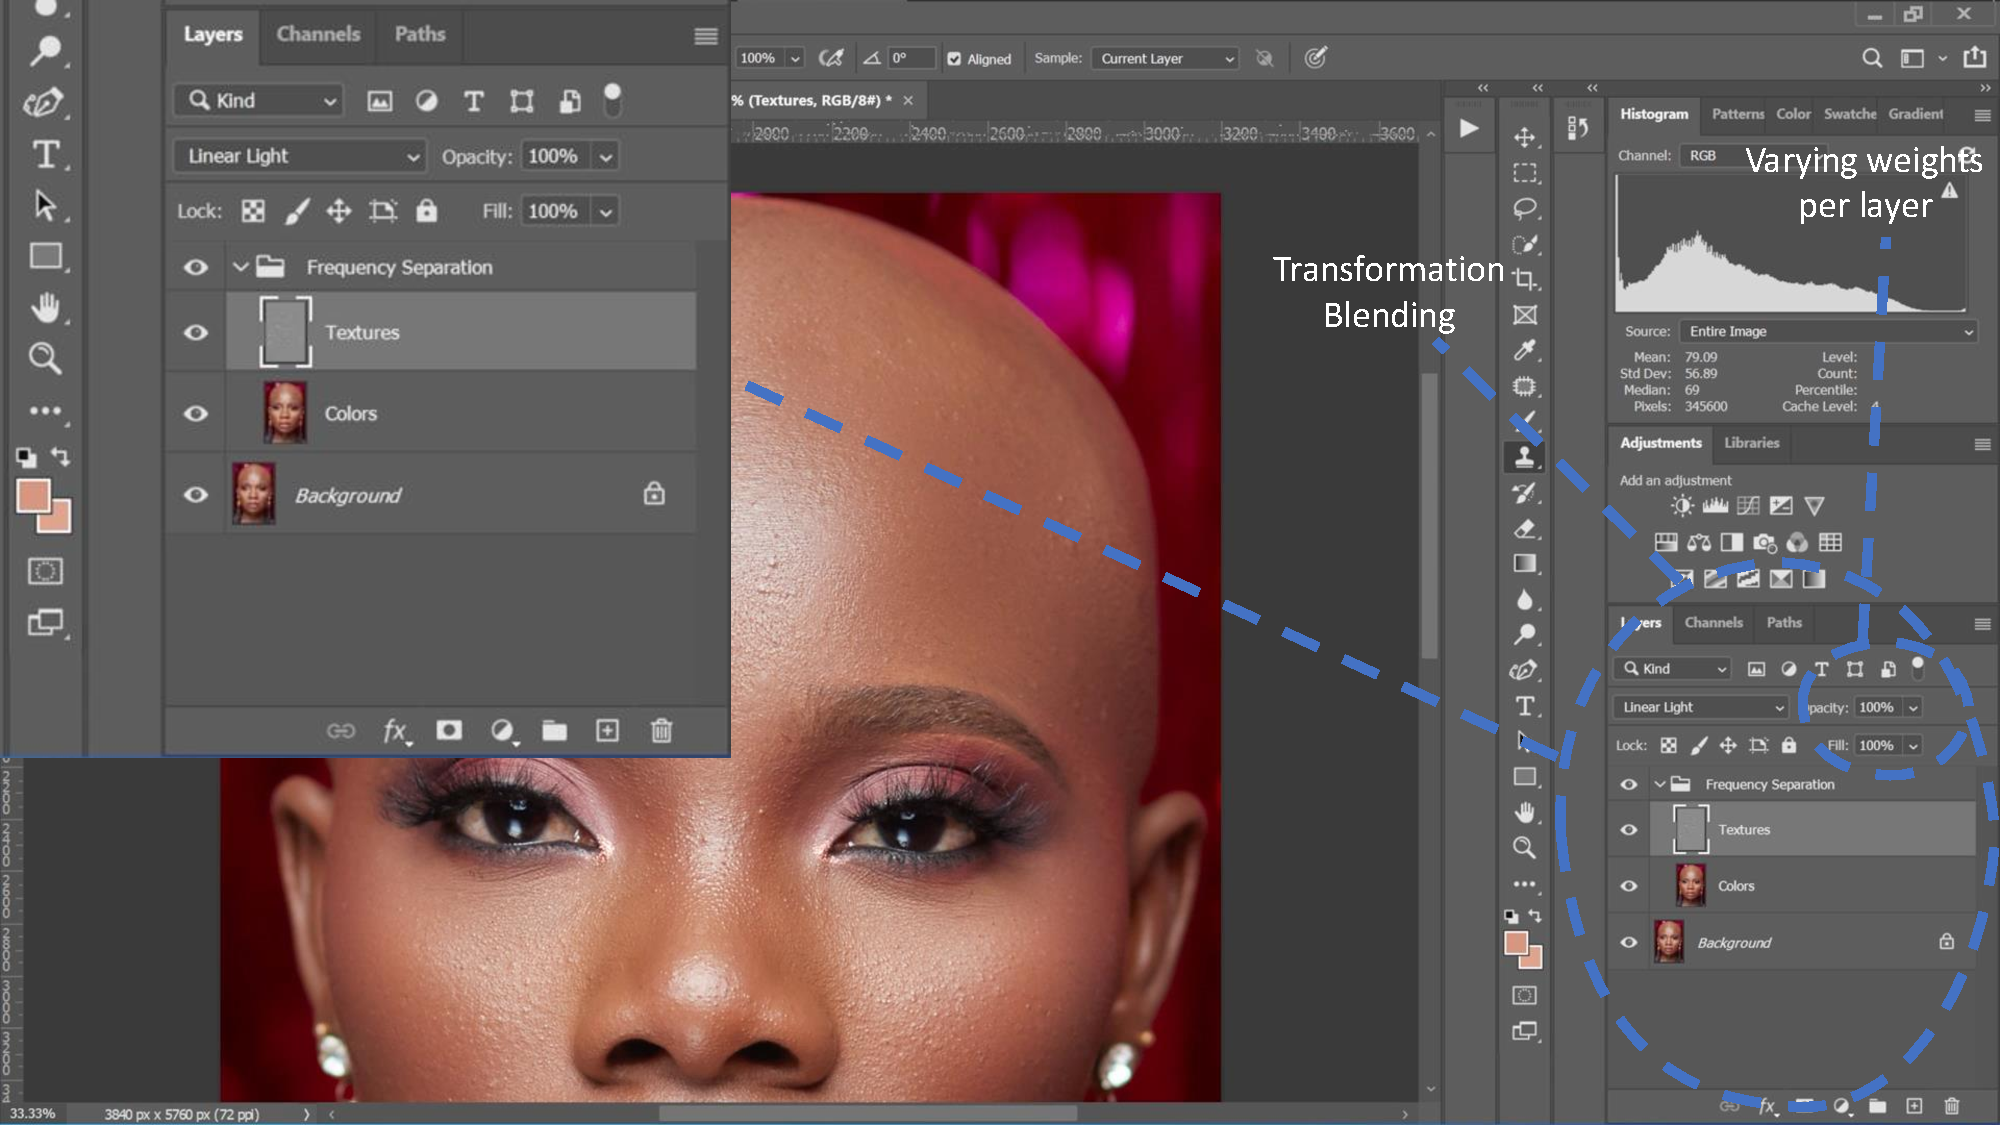
\includegraphics[width=\columnwidth]{Chapters/detail-retouching-figs/PS2.pdf}
    \caption{Artists typically work on separate layers, adjusting various properties, such as texture, colour, and so on. Later, these layers are blended together with their corresponding "opacity" values, shown in the box above the layers.}

\label{fig:PS-all-together}
\end{figure}
\newpage

\item Third, these edits—global and local adjustments—are typically applied in separate layers and then blended using a subjective opacity value. The neural transformation blending with an \gls{MLP} block outputting the weights for each layer replicates the composition of different layers with their corresponding opacity values (Figure \ref{fig:PS-all-together}).

\end{itemize}
Although the professional artist pipelines inspire this work, I will illustrate in the following sections that this new image-to-image mapping representation can replicate the effects of and transfer edits for various filters.
